\section{Evaluierung des Wellenfrontrekonstruktionsalgorithmus}

\subsection{Überblick}
\begin{frame}{Versuchsaufbau}
	\begin{tikzpicture}
		\node at (0,0) {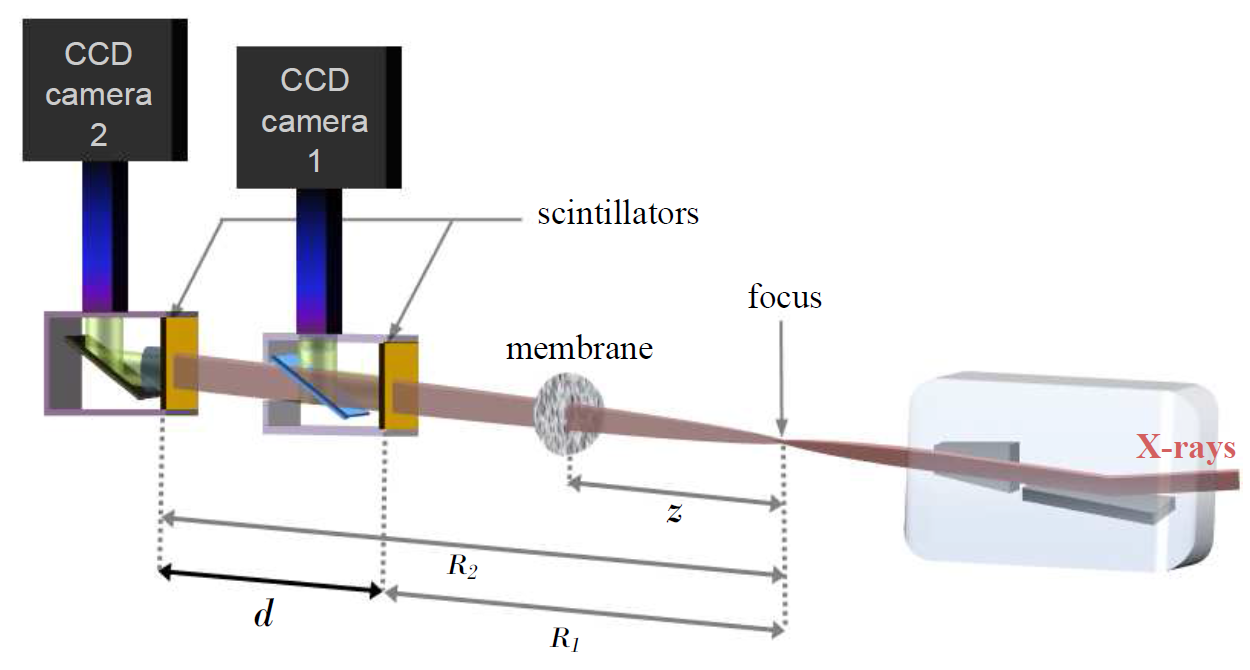
\includegraphics[width=0.98\linewidth]{./img/versuchsaufbau.png}};
		\only<2>{\draw[red, very thick] (2.4, -2.2) rectangle (5.5, -0.2);}
		\only<3>{\draw[red, very thick] (1.2, -1.2) rectangle (1.6, -0.8);}
		\only<4>{\draw[red, very thick] (-1.1, -1.4) rectangle (0.3, 0);}
		
		\only<5>{\draw[red, very thick] (-5.5, 2.9) rectangle (-1.7, -1);}
		\only<6>{\draw[red, very thick] (-4.3, -2.7) rectangle (-2.1, -2);}
		\only<7>{\draw[red, very thick] (-3.3, -1) rectangle (-1.7, 0.1);}
		
		\only<8>{\draw[red, very thick] (-3.6, 1.2) rectangle (-1.9, 2.7);}
		\only<8>{\node at (3.4,0.8) {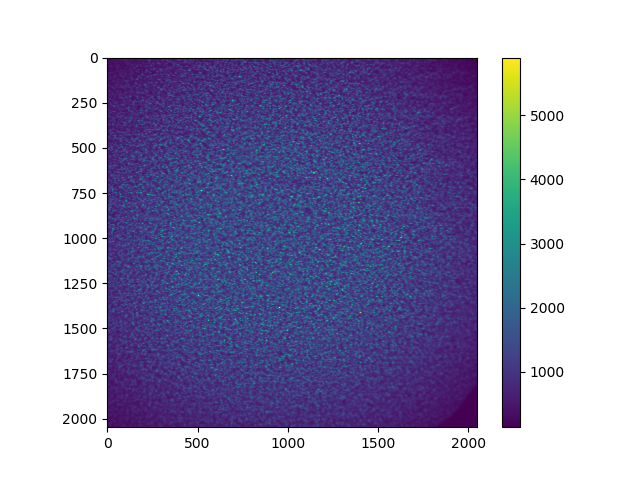
\includegraphics[width=0.5\linewidth]{img/ref_start0001_1-10}};}
		\only<8>{\draw[red, very thick] (1, 2.8) rectangle (5.8, -1.3);}
		\only<8>{\draw[red, very thick] (1, 2.8) -- (-1.9, 2.7);}
		\only<8>{\draw[red, very thick] (1, -1.3) -- (-1.9, 1.2);}
		
		\only<9>{\draw[red, very thick] (-5.3, -0.8) rectangle (-3.7, 0.3);}
		\only<10>{\draw[red, very thick] (-5.5, 1.5) rectangle (-3.8, 2.9);}
		
		\only<10>{\node at (3.4,0.8) {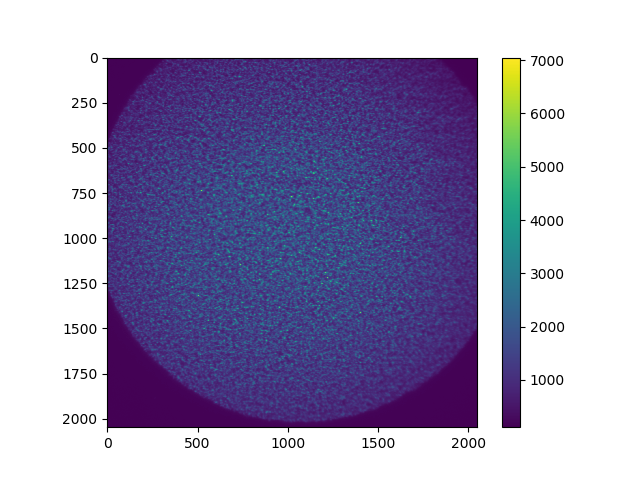
\includegraphics[width=0.5\linewidth]{img/E10001}};}
		\only<10>{\draw[red, very thick] (1, 2.8) rectangle (5.8, -1.3);}
		\only<10>{\draw[red, very thick] (1, 2.8) -- (-3.8, 2.9);}
		\only<10>{\draw[red, very thick] (1, -1.3) -- (-3.8, 1.5);}
	\end{tikzpicture}
\nocite{Ber12}
\nocite{Ber13}
\nocite{Ber15}
{\scriptsize \citeall{Ber15}}
\end{frame}

\begin{frame}{Überblick}
\textbf{Zwei Phasen:}
\begin{itemize}
	\item Initialisierungsphase
	\begin{itemize}
		\item Ermitteln des Kamerafehlers
		\item Bestimmen Ablenkung in verschiedenen Positionen \\
			$\Rightarrow$ Grundlage für Hauptroutine
	\end{itemize}
	\item<2-> Hauptroutine
	\begin{itemize}
		\item Korrigieren von Kamerafehlern ($ \rightarrow $ mit Ausgabe der Initialisierung)
		\item Ablenkung nachverfolgen
		\item Wellenfront rekonstruieren
	\end{itemize}
\end{itemize}
\end{frame}

\begin{frame}{Hauptroutine}
\only<1-5> {
	\begin{tikzpicture}
	\node at (-5,0) {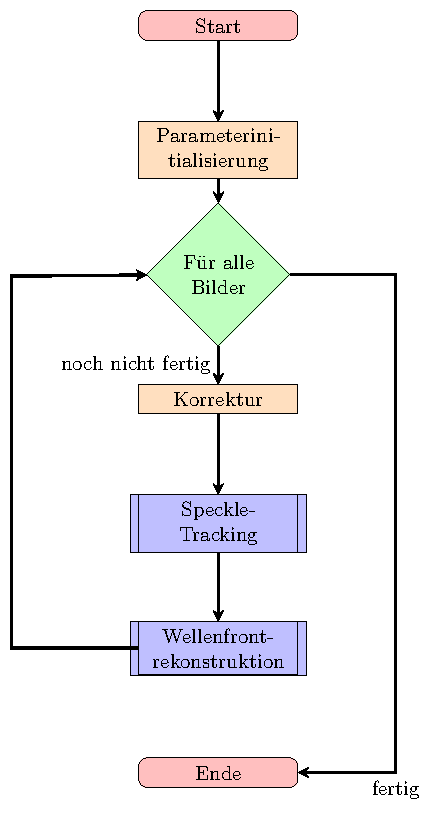
\includegraphics[width=0.35\linewidth]{tex/graph_main}};
	\only<2-4>{\node at (-2,0) {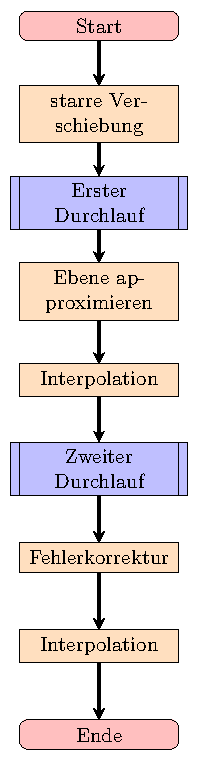
\includegraphics[width=0.17\linewidth]{tex/graph_speckle}}};
	
	\only<2>{\draw[red, very thick] (-5.9, -1.4) rectangle (-4.1, -0.7)};
	\only<2>{\draw[red, very thick] (-4.1, -0.7) -- (-3, 3.7)};
	\only<2>{\draw[red, very thick] (-4.1, -1.4) -- (-3, -3.7)};
	\only<2>{\draw[red, very thick] (-3, -3.7) rectangle (-0.9, 3.7)};
	
	
	\only<3-4>{\draw[red!25, very thick] (-5.9, -1.4) rectangle (-4.1, -0.7)};
	\only<3-4>{\draw[red!25, very thick] (-4.1, -0.7) -- (-3, 3.7)};
	\only<3-4>{\draw[red!25, very thick] (-4.1, -1.4) -- (-3, -3.7)};
	\only<3-4>{\draw[red!25, very thick] (-3, -3.7) rectangle (-0.9, 3.7)};
	
	\only<3>{\draw[red, very thick] (-2.95, 1.4) rectangle (-1.05, 2.07)};
	
	\only<4>{\draw[red, very thick] (-2.95, -1.2) rectangle (-1.05, -0.55)};
	
	\only<5>{\draw[red, very thick] (-5.9, -1.4) rectangle (-4.1, -0.7)};
	\only<5>{\node at (1,2.1) {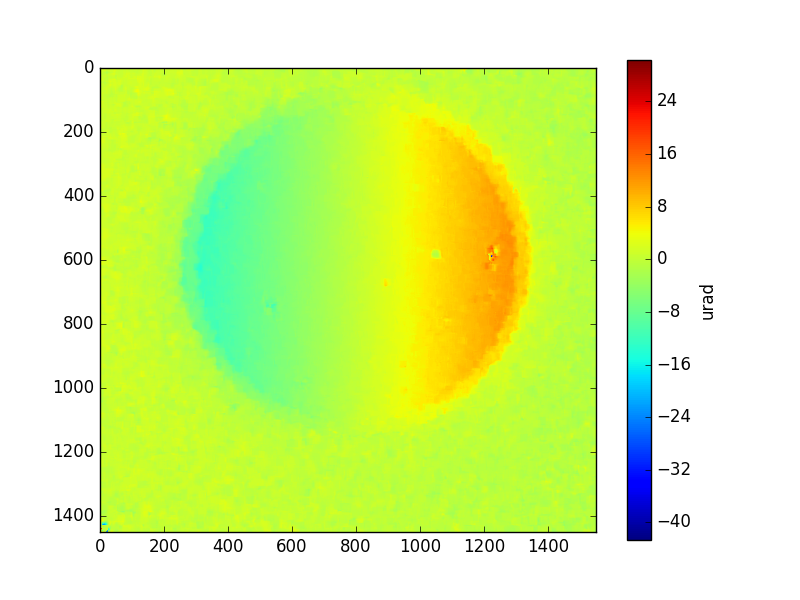
\includegraphics[width=0.4\linewidth]{img/SpeckDisH_E10001_edf_ref_start0001_1-10_edf}}};
	\only<5>{\node at (1,-1.6) {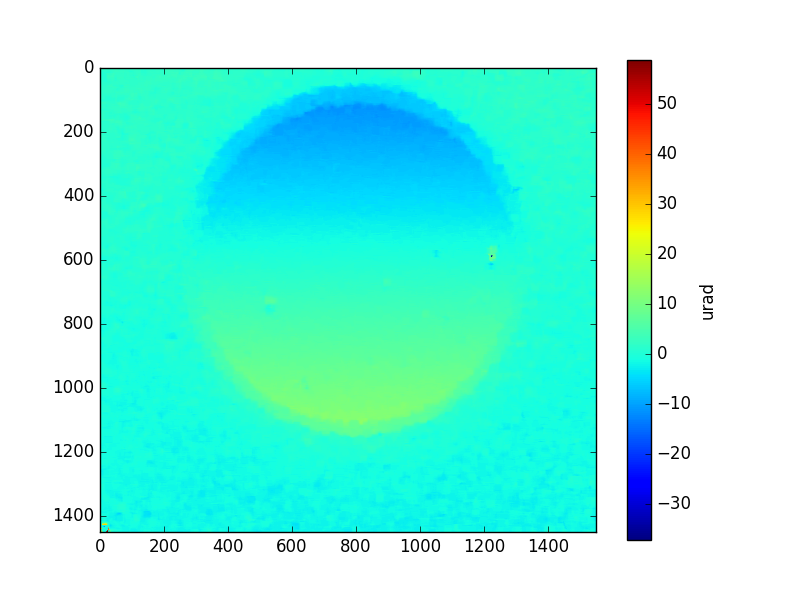
\includegraphics[width=0.4\linewidth]{img/SpeckDisV_E10001_edf_ref_start0001_1-10_edf}}};
	\only<5>{\draw[red, very thick] (-1.2, -3.7) rectangle (2.9, 3.7)};
	\only<5>{\draw[white] (-1, 0.2) rectangle node[black]{Horizontaler Gradient} (2.5, 0.5)};
	\only<5>{\draw[white] (-1, -3.6) rectangle node[black]{Vertikaler Gradient} (2.5, -3.1)};
	\only<5>{\draw[red, very thick] (-4.1, -0.7) -- (-1.2, 3.7)};
	\only<5>{\draw[red, very thick] (-4.1, -1.4) -- (-1.2, -3.7)};
	
	\only<6-7>{\draw[red, very thick] (-5.9, -2.5) rectangle (-4.1, -1.85)};
	\only<6>{\node at (-2,0) {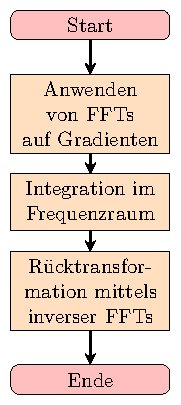
\includegraphics[width=0.17\linewidth]{tex/graph_fc}}};
	
	\only<6>{\draw[red, very thick] (-4.1, -1.85) -- (-3, 2.3)};
	\only<6>{\draw[red, very thick] (-4.1, -2.5) -- (-3, -2.3)};
	\only<6>{\draw[red, very thick] (-3, -2.3) rectangle (-0.9, 2.3)};
	
	\only<7>{\node at (1,0) {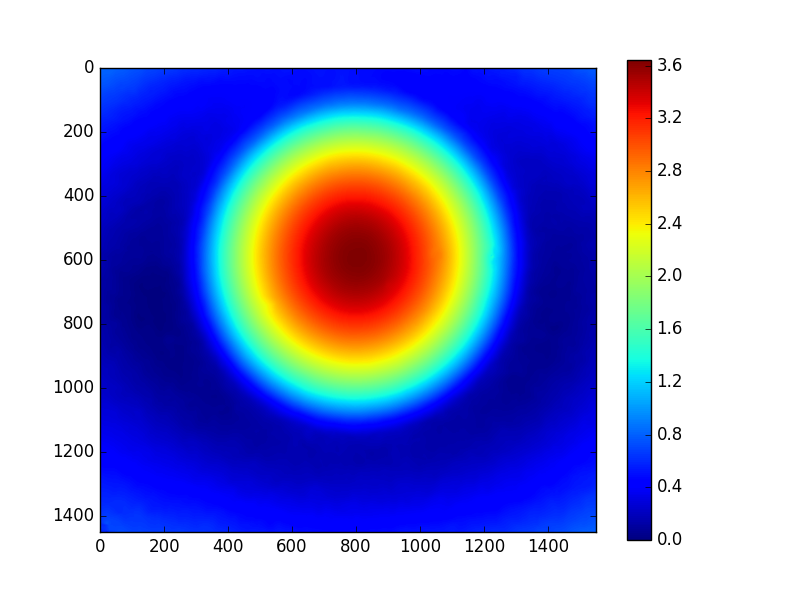
\includegraphics[width=0.6\linewidth]{img/2D_E10001_edf_ref_start0001_1-10_edf}}};
	\only<7>{\draw[red, very thick] (-2, -3) rectangle (3.6, 2.2)};
	\only<7>{\draw[white] (-1, -2.7) rectangle node[black]{Integrierte Gradientenmatrix} (2.5, -2.9)};
	\only<7>{\draw[red, very thick] (-4.1, -1.85) -- (-2, 2.2)};
	\only<7>{\draw[red, very thick] (-4.1, -2.5) -- (-2, -3)};
	\end{tikzpicture}
}
	\only<6-7> {\scalebox{0.9}{
			\begin{tikzpicture}
			\node at (-5,0) {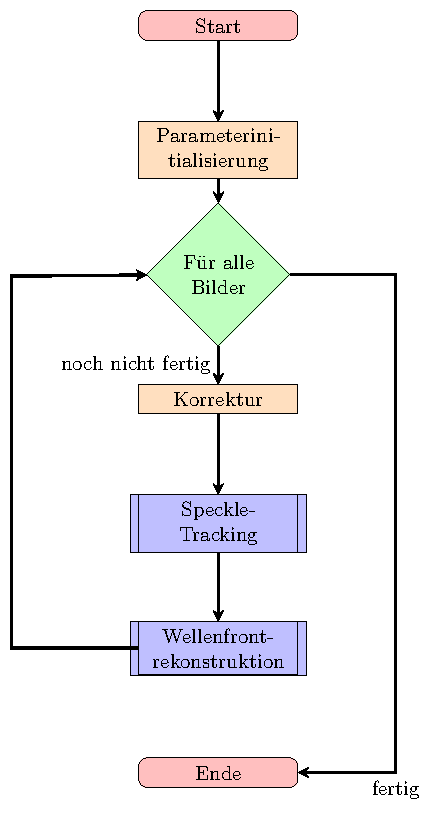
\includegraphics[width=0.35\linewidth]{tex/graph_main}};
			\only<2-4>{\node at (-2,0) {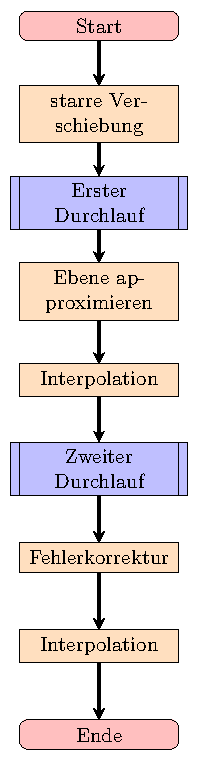
\includegraphics[width=0.17\linewidth]{tex/graph_speckle}}};
			
			\only<2>{\draw[red, very thick] (-5.9, -1.4) rectangle (-4.1, -0.7)};
			\only<2>{\draw[red, very thick] (-4.1, -0.7) -- (-3, 3.7)};
			\only<2>{\draw[red, very thick] (-4.1, -1.4) -- (-3, -3.7)};
			\only<2>{\draw[red, very thick] (-3, -3.7) rectangle (-0.9, 3.7)};
			
			
			\only<3-4>{\draw[red!25, very thick] (-5.9, -1.4) rectangle (-4.1, -0.7)};
			\only<3-4>{\draw[red!25, very thick] (-4.1, -0.7) -- (-3, 3.7)};
			\only<3-4>{\draw[red!25, very thick] (-4.1, -1.4) -- (-3, -3.7)};
			\only<3-4>{\draw[red!25, very thick] (-3, -3.7) rectangle (-0.9, 3.7)};
			
			\only<3>{\draw[red, very thick] (-2.95, 1.4) rectangle (-1.05, 2.07)};
			
			\only<4>{\draw[red, very thick] (-2.95, -1.2) rectangle (-1.05, -0.55)};
			
			\only<5>{\draw[red, very thick] (-5.9, -1.4) rectangle (-4.1, -0.7)};
			\only<5>{\node at (1,2.1) {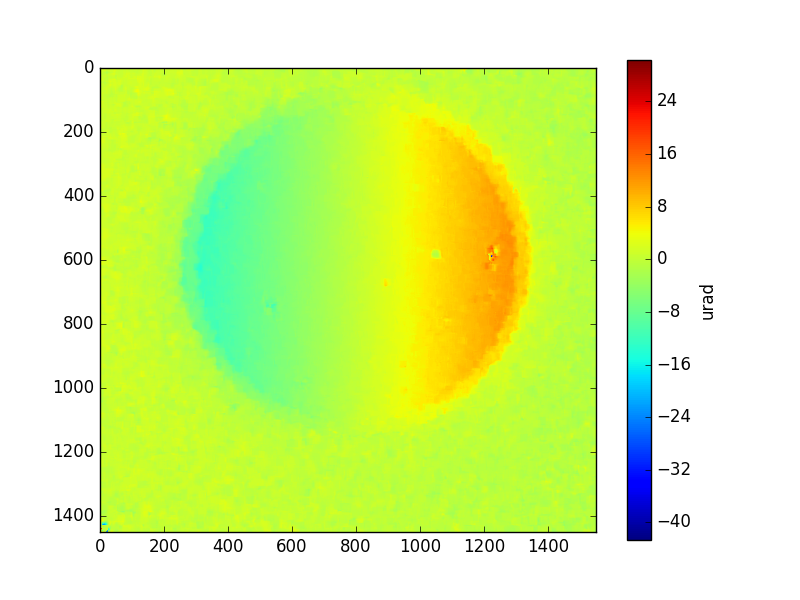
\includegraphics[width=0.4\linewidth]{img/SpeckDisH_E10001_edf_ref_start0001_1-10_edf}}};
			\only<5>{\node at (1,-1.6) {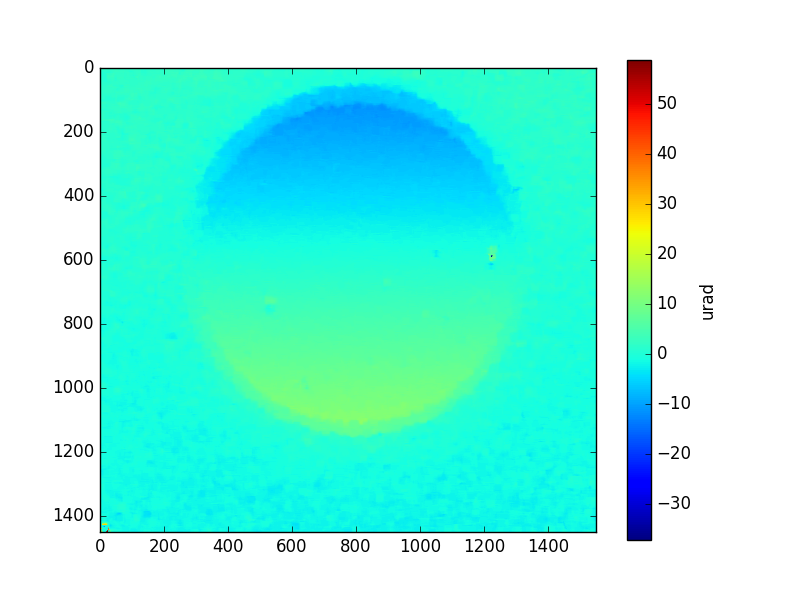
\includegraphics[width=0.4\linewidth]{img/SpeckDisV_E10001_edf_ref_start0001_1-10_edf}}};
			\only<5>{\draw[red, very thick] (-1.2, -3.7) rectangle (2.9, 3.7)};
			\only<5>{\draw[white] (-1, 0.2) rectangle node[black]{Horizontaler Gradient} (2.5, 0.5)};
			\only<5>{\draw[white] (-1, -3.6) rectangle node[black]{Vertikaler Gradient} (2.5, -3.1)};
			\only<5>{\draw[red, very thick] (-4.1, -0.7) -- (-1.2, 3.7)};
			\only<5>{\draw[red, very thick] (-4.1, -1.4) -- (-1.2, -3.7)};
			
			\only<6-7>{\draw[red, very thick] (-5.9, -2.5) rectangle (-4.1, -1.85)};
			\only<6>{\node at (-2,0) {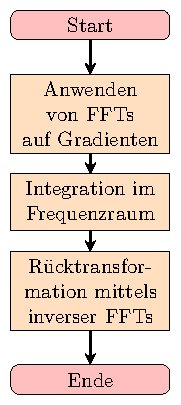
\includegraphics[width=0.17\linewidth]{tex/graph_fc}}};
			
			\only<6>{\draw[red, very thick] (-4.1, -1.85) -- (-3, 2.3)};
			\only<6>{\draw[red, very thick] (-4.1, -2.5) -- (-3, -2.3)};
			\only<6>{\draw[red, very thick] (-3, -2.3) rectangle (-0.9, 2.3)};
			
			\only<7>{\node at (1,0) {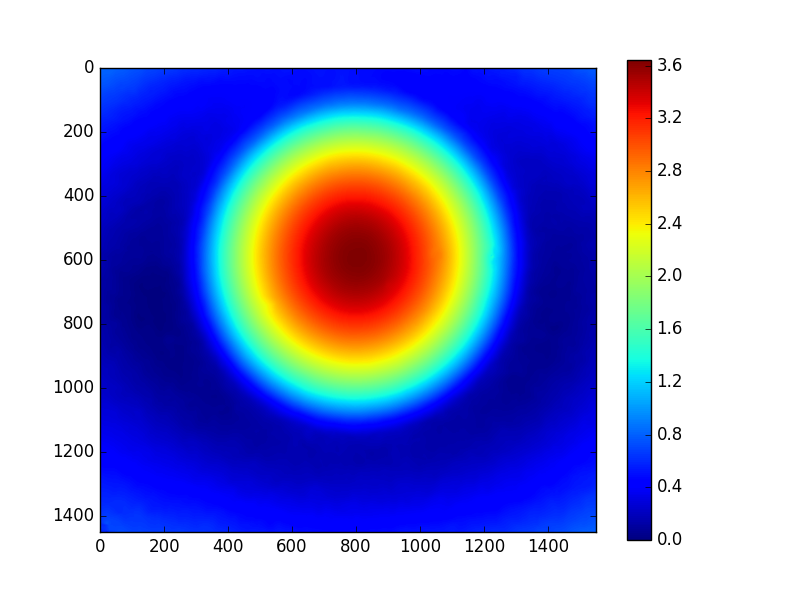
\includegraphics[width=0.6\linewidth]{img/2D_E10001_edf_ref_start0001_1-10_edf}}};
			\only<7>{\draw[red, very thick] (-2, -3) rectangle (3.6, 2.2)};
			\only<7>{\draw[white] (-1, -2.7) rectangle node[black]{Integrierte Gradientenmatrix} (2.5, -2.9)};
			\only<7>{\draw[red, very thick] (-4.1, -1.85) -- (-2, 2.2)};
			\only<7>{\draw[red, very thick] (-4.1, -2.5) -- (-2, -3)};
			\end{tikzpicture}
			\footnote{\citeall{fc88}}
	}}
\end{frame}

\begin{frame}{Initialisierung}
	\begin{center}
		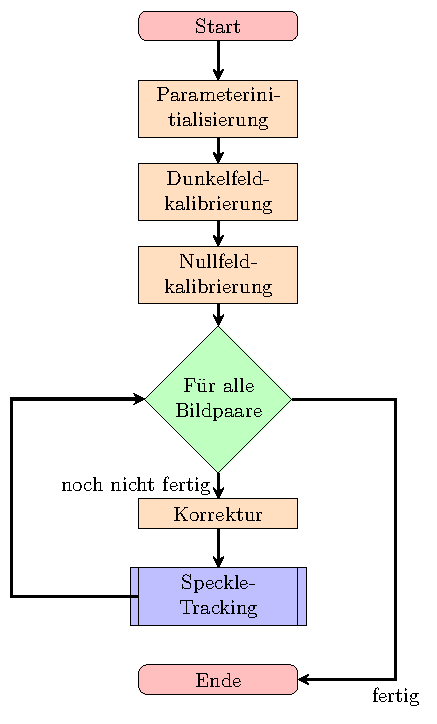
\includegraphics[width=0.4\linewidth]{tex/graph_init}
	\end{center}
\end{frame}

\iffalse

\subsection{Komplexität}
\begin{frame}[allowframebreaks]
\frametitle{Komplexität}
\begin{center}
	$ n $ -- Anzahl der Pixel; $ m $ -- Anzahl der Bilder \\
\end{center}
\textbf{Initialisierung:} \\
\setlength\extrarowheight{5pt}
\begin{center}
	\begin{tabular}{| >{\centering\arraybackslash}m{4cm} | >{\centering\arraybackslash}m{5cm} |}
		\hline
		Untergrund bestimmen & $ \mathcal{O}(m * n) $ \\ \hline
		Nullfeld-Kalibrierung & $ \mathcal{O}(m * n) $ \\ \hline
		Streueffekterkennung & $ \mathcal{O}(m^2 * \frac{n * corrSize * log(corrSize)}{(underSample * gridResol)^2}) \approx \mathcal{O}(m^2 * n^2 * log(n)) $ \\ \hline
	\end{tabular}
\end{center}
\vspace{.5cm}
\textbf{$ \Rightarrow $ Gesamtkomplexität:} $ \approx \mathcal{O}(m^2 * n^2 * log(n)) $

\framebreak

\begin{center}
	$ n $ -- Anzahl der Pixel; $ m $ -- Anzahl der Bilder \\
\end{center}
\textbf{Hauptroutine:} \\
\setlength\extrarowheight{5pt}
\begin{center}
	\begin{tabular}{| >{\centering\arraybackslash}m{4cm} | >{\centering\arraybackslash}m{5cm} |}
		\hline
		Bild-Präprozessierschritte & $ \mathcal{O}(m * n) $ \\ \hline
		Speckle-Tracking & $ \mathcal{O}(m * \frac{n * corrSize * log(corrSize)}{(underSample * gridResol)^2}) \approx \mathcal{O}(m * n^2 * log(n))$ \\ \hline
		Rekonstruktion der Wellenfront & $ \mathcal{O}(m * n * log(n)) $ \\ \hline
	\end{tabular}
\end{center}
\vspace{.5cm}
\textbf{$ \Rightarrow $ Gesamtkomplexität:} $ \approx \mathcal{O}(m * n^2 * log(n)) $
\end{frame}

\fi